 \section{Propuesta}
	
\begin{frame}{Propuesta de solución}
% 	\begin{block}{Herramienta para el desarrollador}
% 	\begin{itemize}
% 	  \item Hacer análisis estático del flujo de información de su aplicación.
% 	  \item Anotaciones en el código fuente.
% 	\end{itemize}
% 	\end{block}
	\begin{figure}[t!]
		\begin{center} 
		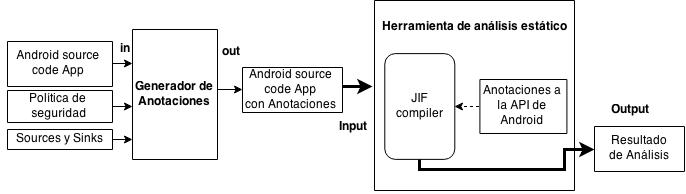
\includegraphics[width=9cm]{desing3Real-2-2.jpg} 
		\end{center}
	\end{figure}
\end{frame}

\begin{frame}{Política de Seguridad}
	\begin{figure}[t!]
		\begin{center} 
		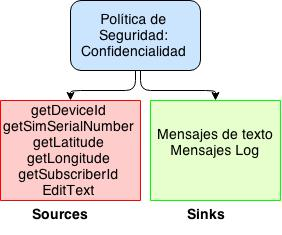
\includegraphics[width=5cm]{Politica.jpg} 
		\end{center}
	\end{figure}
\end{frame}

\begin{frame}{Lineamientos de Anotación}
	\center{Autoridad Máxima}
	\begin{center}
		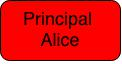
\includegraphics[width=1cm]{Principal.jpg}
	\end{center}
	
		\begin{columns}[c]
			\column{1.5in}
				\begin{center}
	 			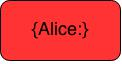
\includegraphics[width=1cm]{high.jpg}
				\end{center}
				Nivel de Seguridad Alto
	 		\column{1.5in}
	 		\begin{center} 
	 			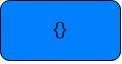
\includegraphics[width=1cm]{low.jpg}
	 			\end{center}
	 			Nivel de Seguridad Bajo\newline
	 			
		\end{columns}
\end{frame}
	
% 	\begin{block}
% % 	\center{Labels de seguridad}
% 	
% % 		\begin{columns}[c]
% % 		\column{1.5}
% % % 			\begin{figure}[t!]
% % % 				\begin{center} 
% % 				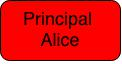
\includegraphics[width=3cm]{Principal.jpg} 
% % % 				\end{center}
% % % 			\end{figure}
% % 			Nivel de seguridad alto
% % 		\end{columns}
% 
% 	\begin{columns}[c]{}
% % 	\column{1.5in}{Autoridad Máxima}
% % 	 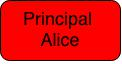
\includegraphics[width=3cm]{Principal.jpg}
% 
% 	 \column{1.5in}
% 	 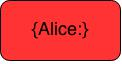
\includegraphics[width=3cm]{high.jpg}\newline
% 	 Nivel de seguridad alto
% 
% 	 \column{1.5in}
% 	 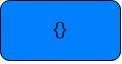
\includegraphics[width=3cm]{low.jpg}\newline
% 	 Nivel de seguridad bajo
% 
% 	\end{columns}
% 	\end{block}
% \end{frame} 

\begin{frame}{Anotaciones a la API}
	\begin{figure}[t!]
		\begin{center} 
		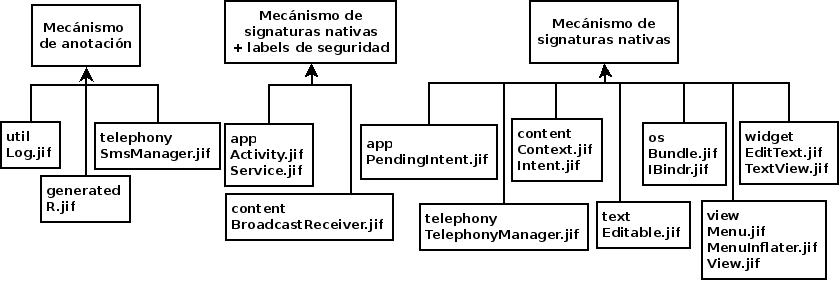
\includegraphics[width=9cm]{annotationsMechanims.jpeg} 
		\end{center}
	\end{figure}
\end{frame}

\begin{frame}{Anotaciones en los aplicativos a analizar}
	
\end{frame}
